\section{Itérations matérielles et analyse des performances}

Afin d'isoler avec précision les goulots d'étranglement du système et de valider l'architecture finale, une série 
de mesures de performances a été menée. L'objectif de cette démarche est de quantifier le temps de transit matériel, 
le temps de transport réseau, puis le temps de traitement de l'image, afin d'établir un bilan "Glass-to-Glass" absolu.

\subsection{Profilage théorique du transport matériel}

\subsubsection{Mesure au cycle d'horloge du traitement MCU (STM32)}
Pour profiler le transfert SPI et l'encapsulation LwIP, le registre matériel ARM CoreSight DWT (\textit{Data Watchpoint and Trace}) 
a été exploité, offrant une résolution de 6.25 nanosecondes.

\begin{lstlisting}[language=C]
dwt_start = DWT->CYCCNT;
// ... [Encapsulation pbuf_alloc et envoi udp_sendto] ...
dwt_end = DWT->CYCCNT;
uint32_t time_us = (dwt_end - dwt_start) / (SystemCoreClock / 1000000);
\end{lstlisting}

L'extraction de cette métrique a révélé qu'avec l'optimisation agressive des files d'attente QoS et la priorité matérielle 
accordée aux paquets vidéo, le temps de traitement MCU est tombé à environ \textbf{0.3 ms par paquet} (contre 0.8 ms initialement), 
minimisant le temps de transit interne du microcontrôleur.

\subsubsection{Bilan de la latence de transport radio pur}
Pour isoler la latence de transmission pure, une architecture à "déclencheur commun" a été mise en place 
(voir Figure \ref{fig:button_latency_test_schematic}). Deux Raspberry Pi 4B (TX et RX) ont été reliées par un bouton poussoir commun. 
Le TX injecte un paquet test via SPI lors de l'appui, et le RX fige son chronomètre haute résolution à la réception.

Les résultats d'un test en rafale (\textit{Burst}) ont donné une moyenne stable de \textbf{10 à 15 ms} par paquet. Ce résultat empirique 
prouve que le transport radio Sub-1 GHz est extrêmement rapide et n'est pas le responsable des lourdes latences observées sur les transmissions 
vidéo standards.

\begin{figure}[htbp]
    \centering
    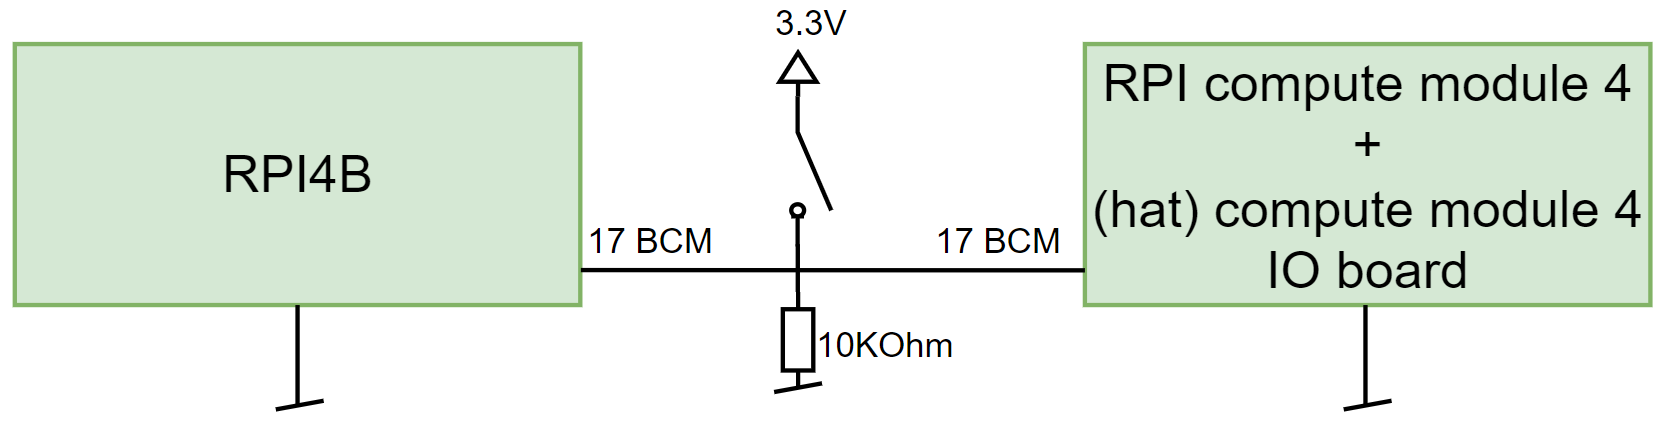
\includegraphics[width=0.8\textwidth]{imgs/button_latency_test_schematic.png}
    \caption{Schéma du système de test de latence matérielle}
    \label{fig:button_latency_test_schematic}
\end{figure}

\subsection{Traque de la latence applicative : Le plafond de verre H.264}
Lors de la première itération du projet (H.264), la latence "Glass-to-Glass" globale s'élevait entre 100 et 140 ms. Sachant que 
le temps de vol matériel pur n'excédait pas 15 ms, plus de 100 millisecondes étaient inexpliquées.

L'approche initiale pour isoler ce problème via un test local (\textit{loopback} sur la même carte) avait mesuré un délai d'encodage 
et de décodage local d'environ 50 à 70 ms. Pour obtenir un diagnostic absolu du goulot d'étranglement, le pont radio Wi-Fi a été totalement 
retiré et remplacé par une connexion réseau filaire directe (câble Ethernet RJ45 direct) reliant l'émetteur et le récepteur.

Le test en Ethernet a confirmé une latence résiduelle incompressible de \textbf{100 à 120 ms}. L'élément radio étant absent, la conclusion 
était claire : la majorité de la latence provenait de la pile logicielle H.264 (buffers du noyau Linux, abstraction V4L2 et surtout la 
répartition et la rétention temporelle inhérente à la reconstruction d'un codec inter-frame). C'est ce diagnostic clé qui a imposé le pivot complet vers le 
MJPEG.

\subsection{Performances et limites de l'architecture finale}

\subsubsection{Comparatif avec un système Broadcast alternatif (DVB-T2)}
Afin de situer les performances de notre architecture par rapport aux standards de transmission numérique du commerce, une étude comparative 
a été menée avec la technologie DVB-T2. Ce système de référence exploitait une carte radio logicielle (SDR BladeRF) pour moduler un 
flux MPEG-TS.

Bien que très robuste en termes de portée, cette approche s'est révélée inexploitable pour le pilotage en temps réel. Les contraintes de multiplexage 
et les importants tampons mémoires des récepteurs standards induisaient une latence "Glass-to-Glass" mesurée entre \textbf{2 et 7 secondes}. Les 
scripts de configuration et les commandes de ce système de référence sont documentés en \textbf{Annexe C}. Ce constat met en lumière la 
pertinence de l'implémentation directe d'un pont SPI-HaLow dédié pour contourner ces goulots d'étranglement industriels.

\subsubsection{Validation matérielle RF et limitations de puissance}
Pour s'assurer que le lien radio exploitait au mieux ses capacités, des tests de puissance d'émission ont été menés à l'aide d'un analyseur de 
spectre en désactivant son mode "low noise" afin de capturer les pics transitoires d'émission lors d'un protocole de \textit{ping flood}. 

Ces mesures physiques ont mis en évidence un comportement inattendu : alors que le module de réception au sol EKH19 émet bien à sa 
puissance maximale de \textbf{20 dBm}, le module d'émission embarqué (EKH05) s'est avéré bridé à une puissance d'émission de seulement 
\textbf{14 dBm}, restant ainsi bien en deçà de sa limite théorique de 26 dBm. Des discussions techniques sont actuellement en cours avec le 
constructeur Morse Micro pour comprendre l'origine de cette limitation logicielle ou matérielle. Bien que cette restriction à 14 dBm 
n'impacte pas la latence à courte portée, elle représente une limite critique pour la portée maximale du drone en vol réel.

\subsubsection{Évaluation empirique de la portée et de la pénétration (NLOS)}
Afin d'évaluer la robustesse physique de la liaison radio HaLow Sub-1 GHz, des tests de transmission ont été réalisés en conditions réelles dans différents environnements d'obstacles, en gardant à l'esprit la limitation physique transitoire à \textbf{14 dBm} de notre module d'émission (TX) :

\begin{table}[htbp]
    \centering
    \renewcommand{\arraystretch}{1.3}
    \begin{tabular}{|l|p{6cm}|p{6.5cm}|}
        \hline
        \textbf{Configuration} & \textbf{Type d'environnement et d'obstacles} & \textbf{Stabilité du flux et Latence} \\
        \hline
        Extérieur (LOS) & Visibilité directe pure sans obstacles & Flux stable jusqu'à \textbf{250 mètres}, latence de 40-50 ms. \\
        \hline
        Intérieur IICT (NLOS) & Traversée de \textbf{2 dalles en béton armé} (sol/plafond) & Image parfaitement stable, pas de décrochage ni de perte de trames. \\
        \hline
        Intérieur IICT limite & Au-delà de 2 étages, obstacles métalliques denses cumulés & Apparition sporadique de macroblocs, puis rupture de la liaison. \\
        \hline
    \end{tabular}
    \caption{Portée utile et comportement de la liaison en mode NLOS}
    \label{tab:nlos_range_test}
\end{table}

Ces essais démontrent de manière éclatante la viabilité de la liaison Sub-1 GHz. Traverser deux dalles complètes en béton au sein des locaux de l'IICT tout en maintenant un débit de 1.53 Mbps est une performance hors de portée pour les systèmes standards 5.8 GHz à puissance égale. L'obtention d'un firmware d'émetteur corrigé permettant d'atteindre les 26 dBm nominaux débloquera des performances de portée NLOS encore supérieures.

\subsubsection{Qualité visuelle en conditions réelles}
La forte compression appliquée (Qualité JPEG fixée au niveau 8) et la résolution de 320x240 pixels représentent le « sweetspot » trouvé empiriquement 
pour maintenir un débit de 1.53 Mbps sans perte de trames. En extérieur, le traitement d'image de l'ISP (lissage automatique du bruit numérique) 
compense la réduction de résolution spatiale. L'image résultante conserve une netteté suffisante pour distinguer précisément les obstacles en vol.

% PLACEHOLDER : Emplacement pour insérer les captures d'écran réelles du flux vidéo (Qualité 8)
\begin{figure}[htbp]
    \centering
    % \includegraphics[width=0.48\textwidth]{imgs/qualite_vol_ext1.jpg}
    % \hspace{0.02\textwidth}
    % \includegraphics[width=0.48\textwidth]{imgs/qualite_vol_ext2.jpg}
    \caption{Captures d'écran du retour vidéo MJPEG (320x240, Qualité 8, 60 FPS) en extérieur}
    \label{fig:qualite_visuelle}
\end{figure}

\subsubsection{Bilan Glass-to-Glass final}
Le système, dans son architecture finale MJPEG et UDP Unicast, a été évalué sur la station de diagnostic en utilisant un écran configuré 
à un taux de rafraîchissement de \textbf{165 Hz}. Ce choix technique est indispensable pour éliminer au maximum la latence liée au temps 
de rafraîchissement, qui pénalise les mesures sur les affichages classiques à 60 Hz.

La méthodologie de métrologie visuelle à base de carrés séquentiels (générant des blocs de couleurs toutes les 5 ms) a permis de collecter 
une série de mesures empiriques exemptes d'erreur de lecture. Les performances globales du système s'établissent ainsi :
\begin{itemize}
    \item \textbf{Latence moyenne :} Entre \textbf{40 ms et 50 ms}.
    \item \textbf{Latence minimale (Pic bas) :} \textbf{30 ms}.
    \item \textbf{Latence maximale (Pic haut) :} \textbf{60 ms} (survenant de manière isolée).
\end{itemize}

L'analyse statistique de ces mesures, représentée graphiquement par la figure \ref{fig:latency_plot}, confirme la disparition de la dérive 
temporelle au fil du temps. Le flux vidéo se maintient largement en dessous du seuil de viabilité fixé par le cahier des charges (80 ms), 
validant ainsi définitivement la faisabilité de l'utilisation du Wi-Fi HaLow pour la transmission vidéo ultra-basse latence.

% Graphique généré à partir de ton fichier CSV de mesures réelles
%\begin{figure}[htbp]
%\centering
%    
\includegraphics[width=0.85\textwidth]{latency_plot.png}
%    \caption{Graphique des mesures empiriques de latence Glass-to-Glass collectées avec le protocole métrologique}
%    \label{fig:latency_plot}
%\end{figure}